\section{Experimental Setup}

\subsection{Controlled Training and Offline Evaluation}

The standard-view dataset contains ten independently generated simulated forest maps, each with 10,000 depth images, camera poses, and a point cloud used only for privileged cost computation. Maps 0--6 are used for training, map 7 for model selection, and maps 8--9 only for final testing. Validation and test ego states are deterministically generated per image.

The main model is trained for 20 epochs from random weights with batch size 16, AdamW, learning rate $1.5\times10^{-4}$, two anchor perturbations, one student perturbation, two accepted refinement steps, and six NFE. Every batch logs total and component losses, gradient norm, target-source fractions, target improvement, and acceptance rate to TensorBoard. The depth backbone is not pretrained. All flow variants contain 11.469 million trainable parameters.

We compare against a direct one-stage lattice regressor retrained on the same map split and budget. For diagnosis, residual-coordinate and physical-coordinate flow variants additionally use a frozen direct policy for initial backbone weights and target proposals. These teacher-guided models quantify the value of teacher information but are not part of the proposed training pipeline. All learned runs use seed 0; training-seed variance is not estimated.

All 20,000 fixed queries from held-out maps 8--9 are evaluated with identical perturbations. Metrics include selected and oracle cost, projected clearance, a 0.6-m collision proxy, score regret, cell switching under small input perturbations, endpoint shift, and full-network latency. Query-level bootstrap intervals are descriptive because samples are nested within only two maps; per-map means are also reported.

\begin{figure*}[t]
    \centering
    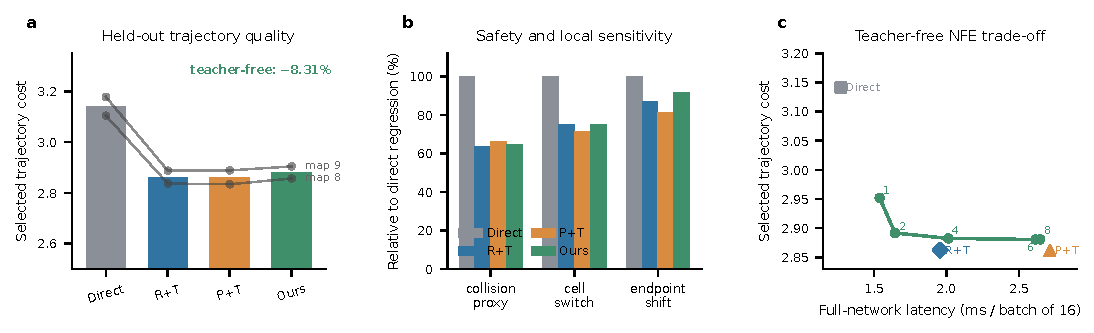
\includegraphics[width=\textwidth]{figures/fig2_offline_results.pdf}
    \caption{Held-out evaluation. (a) Selected cost overall and on each map. R+T and P+T are teacher-guided residual- and physical-coordinate diagnostics; Ours is teacher-free physical flow. (b) Safety and local-sensitivity metrics normalized to direct lattice regression. (c) NFE--latency trade-off for the teacher-free model with six-NFE diagnostic references. All means use 20,000 fixed queries.}
    \label{fig:offline}
\end{figure*}

\subsection{ROS Closed Loop}

Closed-loop trials use the CUDA depth simulator, fifth-order reconstruction, an SO(3) controller, and geometric collision checking against the captured forest point cloud. Simulator seed 3, start $[2,-2,2]$~m, and five goals are fixed across methods. Success requires entering a 1-m goal ball within 60~s; collision is clearance below 0.3~m. Each policy--goal pair restarts from the same state. With five rollouts per configuration on one map, the outcomes are descriptive.

\subsection{LiDAR Perception-Domain Matching}

The real platform has a Livox MID-360 rather than a depth camera. We therefore render a second 100,000-frame dataset with the sensor's elevated field of view: $90^{\circ}$ horizontal and approximately $-7^{\circ}$ to $+52^{\circ}$ vertical, represented by a $+22.5^{\circ}$ optical-axis elevation. The same map split and 20-epoch training protocol are retained. Each dense simulator image is converted to the deployed input domain using one of 120 recorded raw-return masks, one $3\times3$ local hole-fill iteration requiring five valid neighbors, a world-frame $z=2$~m virtual-ceiling projection at stride two, 20-m no-return depth, range noise, and quantization. The ceiling is an image-space sensing prior, not a trajectory-height constraint. Dense depth, point clouds, and ESDFs remain training-only privileged signals.

The deployed model is a separately trained, sensor-matched instance of the same teacher-free architecture. It is exported to FP16 TensorRT with six NFE and runs on an NVIDIA Orin NX. Registered LiDAR points and LIO odometry are projected online to a $96\times160$ depth image; the output terminal state is reconstructed and published to the existing position-command controller.

\subsection{Real-Flight Protocol}

We analyze two independently recorded obstacle-avoidance flights with nominal forward goals of 4 and 8~m. Both use raw minimum-score selection; the continuity selector is disabled. Success is final odometry within 1~m of the commanded goal with no observed physical contact. Bag analysis uses all command-mode odometry and controller samples. For visualization only, accumulated LiDAR returns are voxelized at 8~cm and restricted to $z\in[0.3,2.5]$~m so ground and overhead returns do not obscure obstacles at flight height. Because $n=2$ and no real-flight baseline was run, these trials test feasibility rather than comparative superiority.
